% !TEX program = xelatex
\documentclass[11pt, a4paper]{article}

% ─── Packages ───────────────────────────────────────────────
\usepackage[margin=2.2cm]{geometry}
\usepackage{amsmath, amssymb, amsfonts}
\usepackage{graphicx}
\usepackage{booktabs}
\usepackage{enumitem}
\usepackage{xcolor}
\usepackage{tikz}
\usepackage{float}
\usepackage{caption}
\usepackage{subcaption}
\usepackage{longtable}
\usepackage{multirow}
\usepackage{array}
\usepackage{colortbl}
\usepackage[ruled, vlined, linesnumbered]{algorithm2e}
\usepackage{hyperref}
\usepackage{xeCJK}

\usetikzlibrary{shapes.geometric, arrows.meta, positioning, calc, fit, backgrounds}

% ─── CJK Font ──────────────────────────────────────────────
\setCJKmainfont{SimSun}
\setCJKsansfont{Microsoft YaHei}

% ─── Colors ─────────────────────────────────────────────────
\definecolor{whartonblue}{RGB}{0, 48, 135}
\definecolor{whartonred}{RGB}{166, 25, 46}
\definecolor{lightgray}{RGB}{245, 245, 245}
\definecolor{midgray}{RGB}{180, 180, 180}
\definecolor{darkgreen}{RGB}{34, 139, 34}
\definecolor{btcolor}{RGB}{52, 152, 219}
\definecolor{cvcolor}{RGB}{231, 76, 60}

% ─── Hyperref Setup ─────────────────────────────────────────
\hypersetup{
    colorlinks=true,
    linkcolor=whartonblue,
    urlcolor=whartonblue,
    citecolor=whartonblue,
    pdftitle={WHSDSC 2026 Phase 1 报告},
    pdfauthor={TheIsoLab},
}

% ─── Header ─────────────────────────────────────────────────
\usepackage{fancyhdr}
\pagestyle{fancy}
\fancyhf{}
\fancyhead[L]{\small\textcolor{gray}{WHSDSC 2026 --- 第一阶段}}
\fancyhead[R]{\small\textcolor{gray}{TheIsoLab}}
\fancyfoot[C]{\small\thepage}
\renewcommand{\headrulewidth}{0.4pt}

% ─── Title ──────────────────────────────────────────────────
\title{%
    \vspace{-1cm}
    {\Large\textcolor{whartonblue}{沃顿高中数据科学竞赛 2026 (WHSDSC)}}\\[6pt]
    {\LARGE\textbf{第一阶段：冰球数据分析报告}}\\[4pt]
    {\large 加时赛感知 Bradley-Terry 模型与校准逻辑回归}
}
\author{%
    \textbf{Team TheIsoLab}\\[2pt]
    {\small 工具：Python (pandas, scipy, matplotlib) $\cdot$ AI 协作：Claude + Gemini + Codex}
}
\date{\small 2026 年 2 月}

% ═════════════════════════════════════════════════════════════
\begin{document}
\maketitle
\thispagestyle{fancy}

% ─── Table of Contents ──────────────────────────────────────
\tableofcontents
\vspace{0.5cm}
\hrule
\vspace{0.5cm}

% ═════════════════════════════════════════════════════════════
\section{项目概述}
\label{sec:overview}

\subsection{竞赛背景}
WHSDSC（沃顿高中数据科学竞赛）2026 第一阶段要求选手对 WHL 2025 赛季数据进行冰球数据分析，具体包含四项任务：

\begin{enumerate}[label=\textbf{(\alph*)}]
    \item \textbf{实力排名与胜率预测}：对全部 32 支球队进行实力排名，并预测 16 场第一轮对决的胜负概率。
    \item \textbf{进攻线质量差异}：找出一线与二线进攻线实力差距最大的前 10 支球队。
    \item \textbf{可视化}：用一张 PNG 回答：``阵容均衡的球队是否更强？''
    \item \textbf{方法论报告}：记录完整的分析过程。
\end{enumerate}

\subsection{核心思路}
我们使用\textbf{加时赛感知的 Bradley-Terry 配对比较模型}估计球队潜在实力参数，然后通过\textbf{校准逻辑回归}将实力差转化为胜率预测——5 折交叉验证 Brier 分数达到 \textbf{0.2430}（基线 0.2459）。

% ═════════════════════════════════════════════════════════════
\section{数据处理流程}
\label{sec:data}

\subsection{原始数据概况}
数据集 \texttt{whl\_2025.csv} 包含 \textbf{25,827 条逐行对战记录}，覆盖 \textbf{1,312 场比赛}、\textbf{32 支球队}。每行记录了一场比赛中某一对进攻线/防守组之间的对抗片段：

\begin{itemize}[nosep]
    \item 球队、进球数、期望进球 (xG)、射门数
    \item 进攻线编号（如 \texttt{first\_off}、\texttt{second\_off}）
    \item 防守组编号（如 \texttt{first\_def}、\texttt{second\_def}）
    \item 上冰时间 (TOI，单位：\textbf{秒})、罚时分钟、门将姓名
    \item 是否进入加时赛 (\texttt{went\_ot})
\end{itemize}

\noindent 数据均衡：每支球队恰好进行了 82 场比赛（41 主场 + 41 客场）。

\subsection{处理流程图}

图~\ref{fig:pipeline} 展示了从原始数据到最终输出的完整流水线。

\begin{figure}[H]
\centering
\begin{tikzpicture}[
    block/.style={rectangle, draw=whartonblue, fill=whartonblue!8, rounded corners=4pt,
                  text width=3.1cm, minimum height=1cm, align=center, font=\small},
    output/.style={rectangle, draw=darkgreen, fill=darkgreen!8, rounded corners=4pt,
                   text width=3.1cm, minimum height=0.9cm, align=center, font=\small},
    arrow/.style={-{Stealth[length=3mm]}, thick, color=gray!70},
]
    \node[block] (raw) {原始 CSV\\25,827 行};

    % 左侧：实力估计与胜率预测
    \node[block, below left=1.0cm and 1.1cm of raw] (agg) {比赛级汇总\\(1,312 场)};
    \node[block, below=0.9cm of agg] (bt) {加时赛感知\\Bradley-Terry\\(MLE)};
    \node[block, below=0.9cm of bt] (logistic) {校准\\逻辑回归};
    \node[output, below=0.9cm of logistic] (pred) {\textbf{对决}\\胜率预测};

    % 中间分支：集成评分与排名（BT + 团队特征）
    \node[block, right=1.2cm of agg] (feat) {特征工程\\(xGD, xG\%, PDO)};
    \node[block, below=0.9cm of feat] (ensemble) {集成评分\\(加权 $z$-score)};
    \node[output, below=1.8cm of ensemble] (rank) {\textbf{实力}\\排名};

    % 右侧：进攻线差异分析
    \node[block, below right=1.0cm and 1.1cm of raw] (line) {逐行过滤\\(仅均势对抗)};
    \node[block, below=0.9cm of line] (adj) {防守难度\\校正\\(混杂控制)};
    \node[output, below=1.8cm of adj] (disp) {\textbf{进攻线差异}\\Top 10};

    % Arrows（修正依赖：BT 由比赛结果估计，不依赖特征工程）
    \draw[arrow] (raw) -- (agg);
    \draw[arrow] (raw) -- (line);

    \draw[arrow] (agg) -- (bt);
    \draw[arrow] (bt) -- (logistic);
    \draw[arrow] (logistic) -- (pred);

    \draw[arrow] (agg) -- (feat);
    \draw[arrow] (feat) -- (ensemble);
    \draw[arrow] (bt) -- (ensemble);
    \draw[arrow] (ensemble) -- (rank);

    \draw[arrow] (line) -- (adj);
    \draw[arrow] (adj) -- (disp);
\end{tikzpicture}
\caption{端到端流水线：逐行数据分为两条主线（实力估计与胜率预测、进攻线差异分析），并生成综合实力排名。}
\label{fig:pipeline}
\end{figure}

\subsection{关键预处理步骤}

\begin{enumerate}
    \item \textbf{比赛级汇总}：将每场比赛的进球、xG、射门、TOI、罚时按球队求和，提取二元结果（主队胜 = 1，客队胜 = 0）。
    \item \textbf{平局验证}：确认数据中不存在平局（所有比赛在常规时间或加时赛中都决出了胜负）。流水线若检测到平局会自动报错。
    \item \textbf{TOI 单位校验}：原始 \texttt{toi} 字段单位为\textbf{秒}（每场比赛 TOI 总和中位数 = 3600.00，即 60 分钟）。所有``每 60 分钟''速率计算均除以 3600 而非 60。
    \item \textbf{加时赛标记}：1,312 场比赛中有 288 场（22.0\%）进入了加时赛，这些比赛在 Bradley-Terry 模型中接受特殊处理（见第~\ref{sec:bt} 节）。
\end{enumerate}

\subsection{特征工程}

我们将每场比赛的主客场记录对称堆叠（每场比赛出现两次，每队一次），计算以下团队级指标：

\begin{table}[H]
\centering
\caption{构造特征及其定义}
\label{tab:features}
\begin{tabular}{lll}
\toprule
\textbf{特征} & \textbf{公式} & \textbf{含义} \\
\midrule
xGD/60 & $\displaystyle\frac{xG_{\text{己}} - xG_{\text{对}}}{\text{TOI} / 3600}$ & 每 60 分钟期望净胜球 \\[8pt]
xG 份额 & $\displaystyle\frac{xG_{\text{己}}}{xG_{\text{己}} + xG_{\text{对}}}$ & 己方 xG 占比 \\[8pt]
PDO & $\text{射门命中率} + \text{扑救率}$ & 运气/可持续性指标 \\[4pt]
GSAx/G & $\displaystyle\frac{xGA - GA}{\text{场次}}$ & 预期失球以上扑救数（门将质量） \\[8pt]
xG/射门 & $\displaystyle\frac{xG_{\text{己}}}{\text{射门}_{\text{己}}}$ & 进攻射门质量 \\[8pt]
PIM/G & $\displaystyle\frac{\text{罚时分钟数}}{\text{场次}}$ & 球队纪律性 \\[4pt]
SOS & $\displaystyle\frac{1}{N}\sum_{k} \beta_{\text{对手}_k}$ & 赛程强度（对手 BT 均值） \\
\bottomrule
\end{tabular}
\end{table}

% ═════════════════════════════════════════════════════════════
\section{核心模型：加时赛感知 Bradley-Terry}
\label{sec:bt}

\subsection{为什么选择 Bradley-Terry？}

\textbf{Bradley-Terry (BT) 模型}（Bradley \& Terry, 1952）是估计配对比较中潜在实力的标准模型。每支球队 $i$ 拥有一个潜在实力参数 $\beta_i$，球队 $i$ 击败球队 $j$ 的概率为：

\begin{equation}
\boxed{P(i \text{ 胜 } j) = \sigma(\beta_i - \beta_j) = \frac{e^{\beta_i - \beta_j}}{1 + e^{\beta_i - \beta_j}}}
\label{eq:bt}
\end{equation}

其中 $\sigma(\cdot)$ 是 \textbf{logistic（sigmoid）函数}：
\[
\sigma(x) = \frac{1}{1 + e^{-x}}
\]

\noindent\textbf{关键性质}：
\begin{itemize}[nosep]
    \item 若 $\beta_i > \beta_j$，则 $P(i > j) > 0.5$——实力更强的球队被预测为优势方。
    \item 该模型具有\textit{传递性}：它隐式地控制了对手强度。
    \item 参数在常数平移下不可识别，我们令 $\bar{\beta} = 0$。
\end{itemize}

\subsection{加时赛问题}

图~\ref{fig:ot_reg} 展示了一个关键发现：\textbf{主场优势在加时赛中几乎消失}。

\begin{figure}[H]
    \centering
    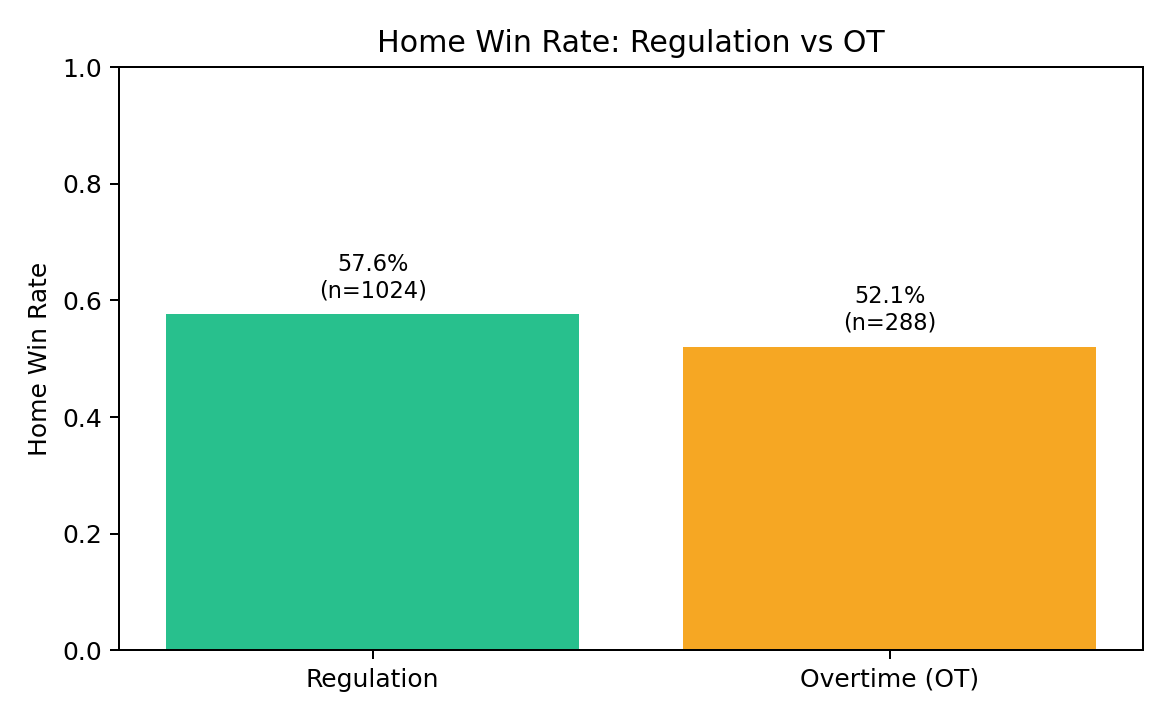
\includegraphics[width=0.55\textwidth]{fig_home_win_ot_reg.png}
    \caption{常规时间主场胜率 57.6\%（$n=1024$） vs.\ 加时赛 52.1\%（$n=288$）。加时赛结果接近``掷硬币''，其中包含的球队实力信号远弱于常规时间胜负。}
    \label{fig:ot_reg}
\end{figure}

如果一场比赛进入加时赛，说明两队在 60 分钟常规时间内旗鼓相当。加时赛胜者很大程度上由运气决定（3 对 3 突然死亡或点球大战）。如果将加时赛胜利与 5--1 常规时间大胜等同对待，会\textbf{向 BT 估计注入噪声}。

\textbf{我们的解决方案}：在似然函数中对加时赛赋予 $w = 0.5$ 的权重：

\begin{equation}
\ell(\boldsymbol{\beta}) = \sum_{k=1}^{K} w_k \Big[ y_k \log \sigma(\beta_{h_k} - \beta_{a_k}) + (1-y_k) \log(1 - \sigma(\beta_{h_k} - \beta_{a_k})) \Big]
\label{eq:likelihood}
\end{equation}

其中：$w_k = 0.5$（加时赛）或 $1.0$（常规时间）；$y_k = 1$ 表示主队获胜；$h_k, a_k$ 分别为主/客队索引。

\subsection{迭代最大似然算法}

我们使用对角 Newton 法最大化对数似然 \eqref{eq:likelihood}：

\begin{algorithm}[H]
\SetAlgoLined
\KwIn{比赛结果 $\{(h_k, a_k, y_k, w_k)\}_{k=1}^K$，球队集合 $\{1,\ldots,N\}$}
\KwOut{实力向量 $\boldsymbol{\beta} \in \mathbb{R}^N$}
$\boldsymbol{\beta} \leftarrow \mathbf{0}$\;
\For{$\text{iter} = 1$ \KwTo $300$}{
    $\mathbf{g} \leftarrow \mathbf{0}$,\quad $\mathbf{H}_{\text{diag}} \leftarrow \mathbf{0}$ \tcp*{梯度与 Hessian 对角线}
    \ForEach{比赛 $k$：主队 $h_k$ vs 客队 $a_k$}{
        $p \leftarrow \sigma(\beta_{h_k} - \beta_{a_k})$ \tcp*{预测概率}
        $\text{residual} \leftarrow w_k(y_k - p)$\;
        $\text{fisher} \leftarrow w_k \cdot p(1-p)$\;
        $g_{h_k} \mathrel{+}= \text{residual}$;\quad $g_{a_k} \mathrel{-}= \text{residual}$\;
        $H_{h_k} \mathrel{-}= \text{fisher}$;\quad $H_{a_k} \mathrel{-}= \text{fisher}$\;
    }
    $\boldsymbol{\delta} \leftarrow -\mathbf{g} \,/\, \mathbf{H}_{\text{diag}}$ \tcp*{Newton 步长（逐元素）}
    $\boldsymbol{\delta} \leftarrow \boldsymbol{\delta} - \overline{\delta}$ \tcp*{中心化：保持 $\sum \beta_i = 0$}
    $\boldsymbol{\beta} \leftarrow \boldsymbol{\beta} + 0.5 \cdot \boldsymbol{\delta}$ \tcp*{阻尼更新（$\nu = 0.5$）}
    \lIf{$\max(|\boldsymbol{\delta}|) < 10^{-8}$}{\textbf{收敛退出}}
}
$\boldsymbol{\beta} \leftarrow \boldsymbol{\beta} - \overline{\beta}$ \tcp*{最终中心化}
\Return{$\boldsymbol{\beta}$}
\caption{加时赛感知 Bradley-Terry 迭代 MLE 算法}
\label{alg:bt}
\end{algorithm}

\noindent\textbf{收敛性}：算法通常在约 30 次迭代内收敛（远低于 300 次上限）。阻尼因子 $\nu = 0.5$ 防止过冲。

% ═════════════════════════════════════════════════════════════
\section{胜率预测：校准逻辑回归}
\label{sec:logistic}

\subsection{模型公式}

原始 BT 概率（公式~\ref{eq:bt}）可能存在校准偏差，因为 BT 模型没有主场优势截距项。我们通过逻辑回归添加校准层：

\begin{equation}
\boxed{P(\text{主队胜}) = \sigma\!\big(\alpha + \gamma \cdot (\beta_{\text{主}} - \beta_{\text{客}})\big)}
\label{eq:logistic}
\end{equation}

\begin{itemize}[nosep]
    \item $\alpha$ = 截距，捕获\textbf{主场优势}（$\alpha = 0.2724 \Rightarrow \sigma(0.2724) = 56.8\%$）
    \item $\gamma$ = 缩放系数（$\gamma = 0.9350$）
\end{itemize}

参数通过 Nelder-Mead 最小化负对数似然求解，预测值\textbf{裁剪至 $[0.01, 0.99]$} 以防极端概率导致 log-loss 爆炸。

\subsection{5 折交叉验证方案}

为了诚实评估预测性能，我们使用 5 折 CV，其中一个关键细节是：\textbf{每折中 BT 实力参数从零重新估计}，仅使用训练数据。

\begin{figure}[H]
\centering
\begin{tikzpicture}[
    fold/.style={rectangle, minimum width=1.8cm, minimum height=0.5cm, font=\small},
    train/.style={fold, fill=btcolor!25, draw=btcolor},
    test/.style={fold, fill=cvcolor!25, draw=cvcolor},
]
    \foreach \i in {1,...,5} {
        \node at (-1.2, -\i*0.7) {\small 第 \i 折:};
    }
    \foreach \i in {1,...,5} {
        \foreach \j in {1,...,5} {
            \ifnum\i=\j
                \node[test] at (\j*2, -\i*0.7) {\textcolor{cvcolor}{测试}};
            \else
                \node[train] at (\j*2, -\i*0.7) {\textcolor{btcolor}{训练}};
            \fi
        }
    }
    \draw[-{Stealth}, thick, gray] (11, -1.5) -- (11, -3.5)
        node[midway, right, font=\small, text width=2.6cm] {BT + 逻辑回归\\每折重拟合\\（零泄漏）};
\end{tikzpicture}
\caption{5 折交叉验证示意图：每折均在训练集上重新拟合 BT 与逻辑回归，确保零数据泄漏。}
\label{fig:cv}
\end{figure}

\subsection{评估结果}

\begin{table}[H]
\centering
\caption{模型对比：5 折交叉验证结果}
\label{tab:cv}
\begin{tabular}{lccc}
\toprule
\textbf{模型} & \textbf{准确率} & \textbf{Log-Loss} & \textbf{Brier 分数} \\
\midrule
基线（主队胜率 = 56.4\%） & 56.4\% & 0.6849 & 0.2459 \\
\textbf{加时赛感知 BT 逻辑回归} & \textbf{57.0\% $\pm$ 3.2\%} & \textbf{0.6797} & \textbf{0.2430} \\
\bottomrule
\end{tabular}
\end{table}

\noindent\textbf{指标解读}：
\begin{itemize}
    \item \textbf{准确率}（57.0\%）：在随机 5 折 CV 中，相比``永远预测主队胜''基线（56.4\%）仅有小幅提升，应按有限提升解读。
    \item \textbf{Log-Loss}（0.6797）：衡量概率预测的置信度质量。越低越好。
    \item \textbf{Brier 分数}（0.2430）：概率预测的均方误差。在随机 CV 中相对基线约下降 1.2\%，属于有限但有用的校准改善。
    \item \textbf{ID-order 压力测试（非真实时序）}：按数值 \texttt{game\_id} 排序的压力测试中，BT 在三项指标上均劣于主场胜率基线（准确率 54.7\% vs 56.2\%，Log-Loss 0.7047 vs 0.6860，Brier 0.2524 vs 0.2464）。由于该模拟数据中的 \texttt{game\_id} 顺序不保证等于真实时间顺序，我们将其视为偏保守的鲁棒性检查，而非部署失败证据。
\end{itemize}

\subsection{概率校准}

校准衡量预测概率与实际结果的一致性。我们使用\textbf{折外 (OOF) 预测}计算校准分箱，防止乐观偏差。
为避免小样本带来的波动，我们仅报告样本量不少于 10 场的分箱。

\begin{table}[H]
\centering
\caption{折外预测校准表。校准良好的模型应满足``预测 $\approx$ 观测''。}
\label{tab:calibration}
\begin{tabular}{cccc}
\toprule
\textbf{分箱中心} & \textbf{平均预测值} & \textbf{实际胜率} & \textbf{样本量 $N$} \\
\midrule
0.31 & 0.334 & 0.407 & 86 \\
0.44 & 0.447 & 0.512 & 297 \\
0.56 & 0.565 & 0.532 & 504 \\
0.69 & 0.680 & 0.666 & 353 \\
0.81 & 0.790 & 0.712 & 66 \\
\bottomrule
\end{tabular}
\end{table}

\noindent 模型在 0.44--0.69 范围内校准良好。在高端（预测 0.79，实际 0.71）存在\textbf{过度自信}，这是已知的局限性（见第~\ref{sec:limitations} 节）。

% ═════════════════════════════════════════════════════════════
\section{集成实力排名}
\label{sec:rankings}

\subsection{综合评分构造}

我们使用五项指标的\textbf{加权 $z$-score 集成}进行排名：

\begin{equation}
\text{综合分}_i = \sum_{m=1}^{5} w_m \cdot z_{i,m}, \qquad
z_{i,m} = \frac{x_{i,m} - \bar{x}_m}{\sigma_m}
\label{eq:composite}
\end{equation}

\begin{table}[H]
\centering
\caption{集成权重分配及理由}
\label{tab:weights}
\begin{tabular}{lcl}
\toprule
\textbf{指标} & \textbf{权重} & \textbf{理由} \\
\midrule
BT 实力值 & 40\% & 核心潜在质量度量，自动控制对手强度 \\
xGD/60 & 30\% & 过程导向指标，比实际进球更稳定 \\
xG 份额 & 10\% & 相对进攻优势 \\
净胜球/场 & 10\% & 已实现结果（非仅期望值） \\
胜率 & 10\% & 竞技结果的直接衡量 \\
\bottomrule
\end{tabular}
\end{table}

\subsection{权重鲁棒性}

我们测试了四种权重方案（含最终方案）：BT 独占（100\%）、均等（各 20\%）、xG 倾斜（xGD/60 占 50\%）等。所有方案之间的 Spearman 秩相关系数为 \textbf{0.81--1.00}。前 6 名中有 \textbf{5 支球队}在所有方案中保持一致，说明头部排名总体稳健但并非完全不受权重影响。该结果现由 \texttt{phase1\_submit.py} 自动生成的内部证据文件 \texttt{output/submission/ranking\_weight\_sensitivity.md} 复核。

\subsection{Top 10 排名}

\begin{table}[H]
\centering
\caption{实力排名（32 队中前 10 名）。完整排名见 CSV 提交文件。}
\label{tab:rankings}
\begin{tabular}{clccccccc}
\toprule
\textbf{\#} & \textbf{球队} & \textbf{综合分} & \textbf{BT} & \textbf{xGD/60} & \textbf{xG\%} & \textbf{胜率} & \textbf{GSAx/G} & \textbf{SOS} \\
\midrule
1  & Brazil      & 2.073 & 0.940 & 0.599 & .551 & .707 & +0.40 & $-$0.050 \\
2  & Thailand    & 1.612 & 0.484 & 0.865 & .571 & .610 & $-$0.32 & $-$0.029 \\
3  & Netherlands & 1.535 & 0.641 & 0.472 & .546 & .659 & +0.34 & $-$0.028 \\
4  & Pakistan    & 1.296 & 0.424 & 0.611 & .549 & .598 & +0.26 & $-$0.026 \\
5  & Peru        & 1.273 & 0.532 & 0.340 & .532 & .634 & +0.45 & $-$0.020 \\
6  & China       & 0.915 & 0.282 & 0.411 & .537 & .573 & +0.34 & $-$0.010 \\
7  & Panama      & 0.653 & 0.267 & 0.190 & .516 & .561 & +0.35 & $-$0.017 \\
8  & India       & 0.633 & 0.396 & 0.016 & .501 & .598 & +0.55 & $-$0.027 \\
9  & UK          & 0.453 & $-$0.012 & 0.424 & .535 & .476 & +0.35 & +0.006 \\
10 & Guatemala   & 0.292 & 0.021 & 0.270 & .523 & .512 & $-$0.04 & $-$0.002 \\
\bottomrule
\end{tabular}
\end{table}

\noindent \textbf{关键洞察}：
\begin{itemize}[nosep]
    \item \textbf{Brazil}：以最高 BT 实力值（0.940）和胜率（70.7\%）独占鳌头。
    \item \textbf{Thailand}：凭借联盟最佳 xGD/60（0.865）位居第二，但 GSAx 为负（门将偏弱）。
    \item \textbf{India}（第 8）：拥有最佳 GSAx/G（+0.55）但 xGD 平平，说明强大门将掩盖了较弱的进攻。
\end{itemize}

% ═════════════════════════════════════════════════════════════
\section{对决胜率预测}
\label{sec:matchups}

使用校准逻辑回归模型（公式~\ref{eq:logistic}），我们预测第一轮 16 场对决：

\begin{table}[H]
\centering
\caption{第一轮对决预测。所有 16 场比赛均预测主队获胜（主场优势效应）。}
\label{tab:matchups}
\begin{tabular}{clllc}
\toprule
\textbf{场次} & \textbf{主队} & \textbf{客队} & \textbf{主队胜率} & \textbf{置信度} \\
\midrule
1  & Brazil      & Kazakhstan    & 85.2\% & 高 \\
2  & Netherlands & Mongolia      & 81.6\% & 高 \\
3  & Peru        & Rwanda        & 79.4\% & 高 \\
4  & Thailand    & Oman          & 73.3\% & 中 \\
5  & Pakistan    & Germany       & 71.2\% & 中 \\
6  & India       & USA           & 72.1\% & 中 \\
7  & Panama      & Switzerland   & 68.8\% & 中 \\
8  & Iceland     & Canada        & 67.4\% & 中 \\
9  & China       & France        & 66.9\% & 中 \\
10 & Philippines & Morocco       & 64.5\% & 低 \\
11 & Ethiopia    & Saudi Arabia  & 64.0\% & 低 \\
12 & Singapore   & New Zealand   & 59.1\% & 低 \\
13 & Guatemala   & South Korea   & 59.7\% & 低 \\
14 & UK          & Mexico        & 60.5\% & 低 \\
15 & Vietnam     & Serbia        & 54.1\% & 五五开 \\
16 & Indonesia   & UAE           & 63.3\% & 低 \\
\bottomrule
\end{tabular}
\end{table}

\noindent 置信度分级：高（$>$75\%）、中（65--75\%）、低（55--65\%）、五五开（$<$55\%）。

% ═════════════════════════════════════════════════════════════
\section{进攻线质量差异分析}
\label{sec:disparity}

\subsection{方法}

我们用一线与二线每 60 分钟 xG 的\textbf{比值}衡量进攻线质量差异：

\begin{equation}
\text{差异比} = \frac{\text{xG/60}_{\text{一线}}}{\text{xG/60}_{\text{二线}}}
\end{equation}

比值为 1.0 表示完全均衡；$> 1.0$ 表示球队过度依赖一线。

\textbf{关键校正}：原始 xG/60 受防守对位质量的混杂影响。我们按对位防守组层级（\texttt{first\_def} vs \texttt{second\_def}）计算\textbf{防守难度因子}并进行归一化；这是一种分层校正，而非基于具体球队防守实力的完全校正：

\begin{equation}
\text{校正 xG/60}_{\text{线}} = \frac{\text{原始 xG/60}_{\text{线}}}{\text{防守难度因子}_{\text{对位防守组}}}
\end{equation}

其中防守难度因子 = 该防守组层级（1 对或 2 对）的 xGA/60 与联盟平均值之比。

\textbf{数据过滤}：仅保留均势对抗（1/2 线进攻 vs.\ 1/2 对防守组），排除强打、少打和空门时段。

\subsection{结果}

\begin{table}[H]
\centering
\caption{校正后进攻线差异排名前 10}
\label{tab:disparity}
\begin{tabular}{clccc}
\toprule
\textbf{\#} & \textbf{球队} & \textbf{一线校正 xG/60} & \textbf{二线校正 xG/60} & \textbf{校正比值} \\
\midrule
1  & USA          & 2.730 & 1.993 & 1.369 \\
2  & Guatemala    & 2.821 & 2.070 & 1.363 \\
3  & Saudi Arabia & 2.244 & 1.654 & 1.357 \\
4  & UAE          & 1.998 & 1.476 & 1.354 \\
5  & France       & 2.559 & 1.901 & 1.346 \\
6  & Iceland      & 2.589 & 1.961 & 1.321 \\
7  & Singapore    & 2.635 & 2.101 & 1.254 \\
8  & New Zealand  & 2.441 & 1.975 & 1.236 \\
9  & Peru         & 2.391 & 1.983 & 1.206 \\
10 & Panama       & 2.545 & 2.120 & 1.201 \\
\bottomrule
\end{tabular}
\end{table}

% ═════════════════════════════════════════════════════════════
\section{提交可视化：阵容均衡 vs.\ 球队实力}
\label{sec:viz}

提交可视化（图~\ref{fig:scatter}）直接回答赛事专员的问题：\textbf{``进攻阵容更均衡的球队是否表现更好？''}

\begin{figure}[H]
    \centering
    
\includegraphics[width=0.82\textwidth]{../output/final_submission/TheIsoLab.png}
    \caption{校正进攻线差异（x 轴） vs.\ 综合实力评分（y 轴）。Pearson $r = -0.031$，$R^2 = 0.001$。\textbf{结论}：不存在显著线性关系——球队通过多样化的阵容策略取得成功。}
    \label{fig:scatter}
\end{figure}

\noindent\textbf{设计选择}：
\begin{itemize}[nosep]
    \item \textbf{色盲友好}：viridis 色图（感知均匀，对色觉缺陷安全）。
    \item \textbf{标注}：前 5 名和后 3 名球队加标签，便于快速识别。
    \item \textbf{统计叠加}：线性趋势线、Pearson $r$ 和 $R^2$，提供定量评估。
\end{itemize}

% ═════════════════════════════════════════════════════════════
\section{完整分析仪表盘}
\label{sec:dashboard}

图~\ref{fig:dashboard} 展示了完整的 5 面板分析仪表盘。

\begin{figure}[H]
    \centering
    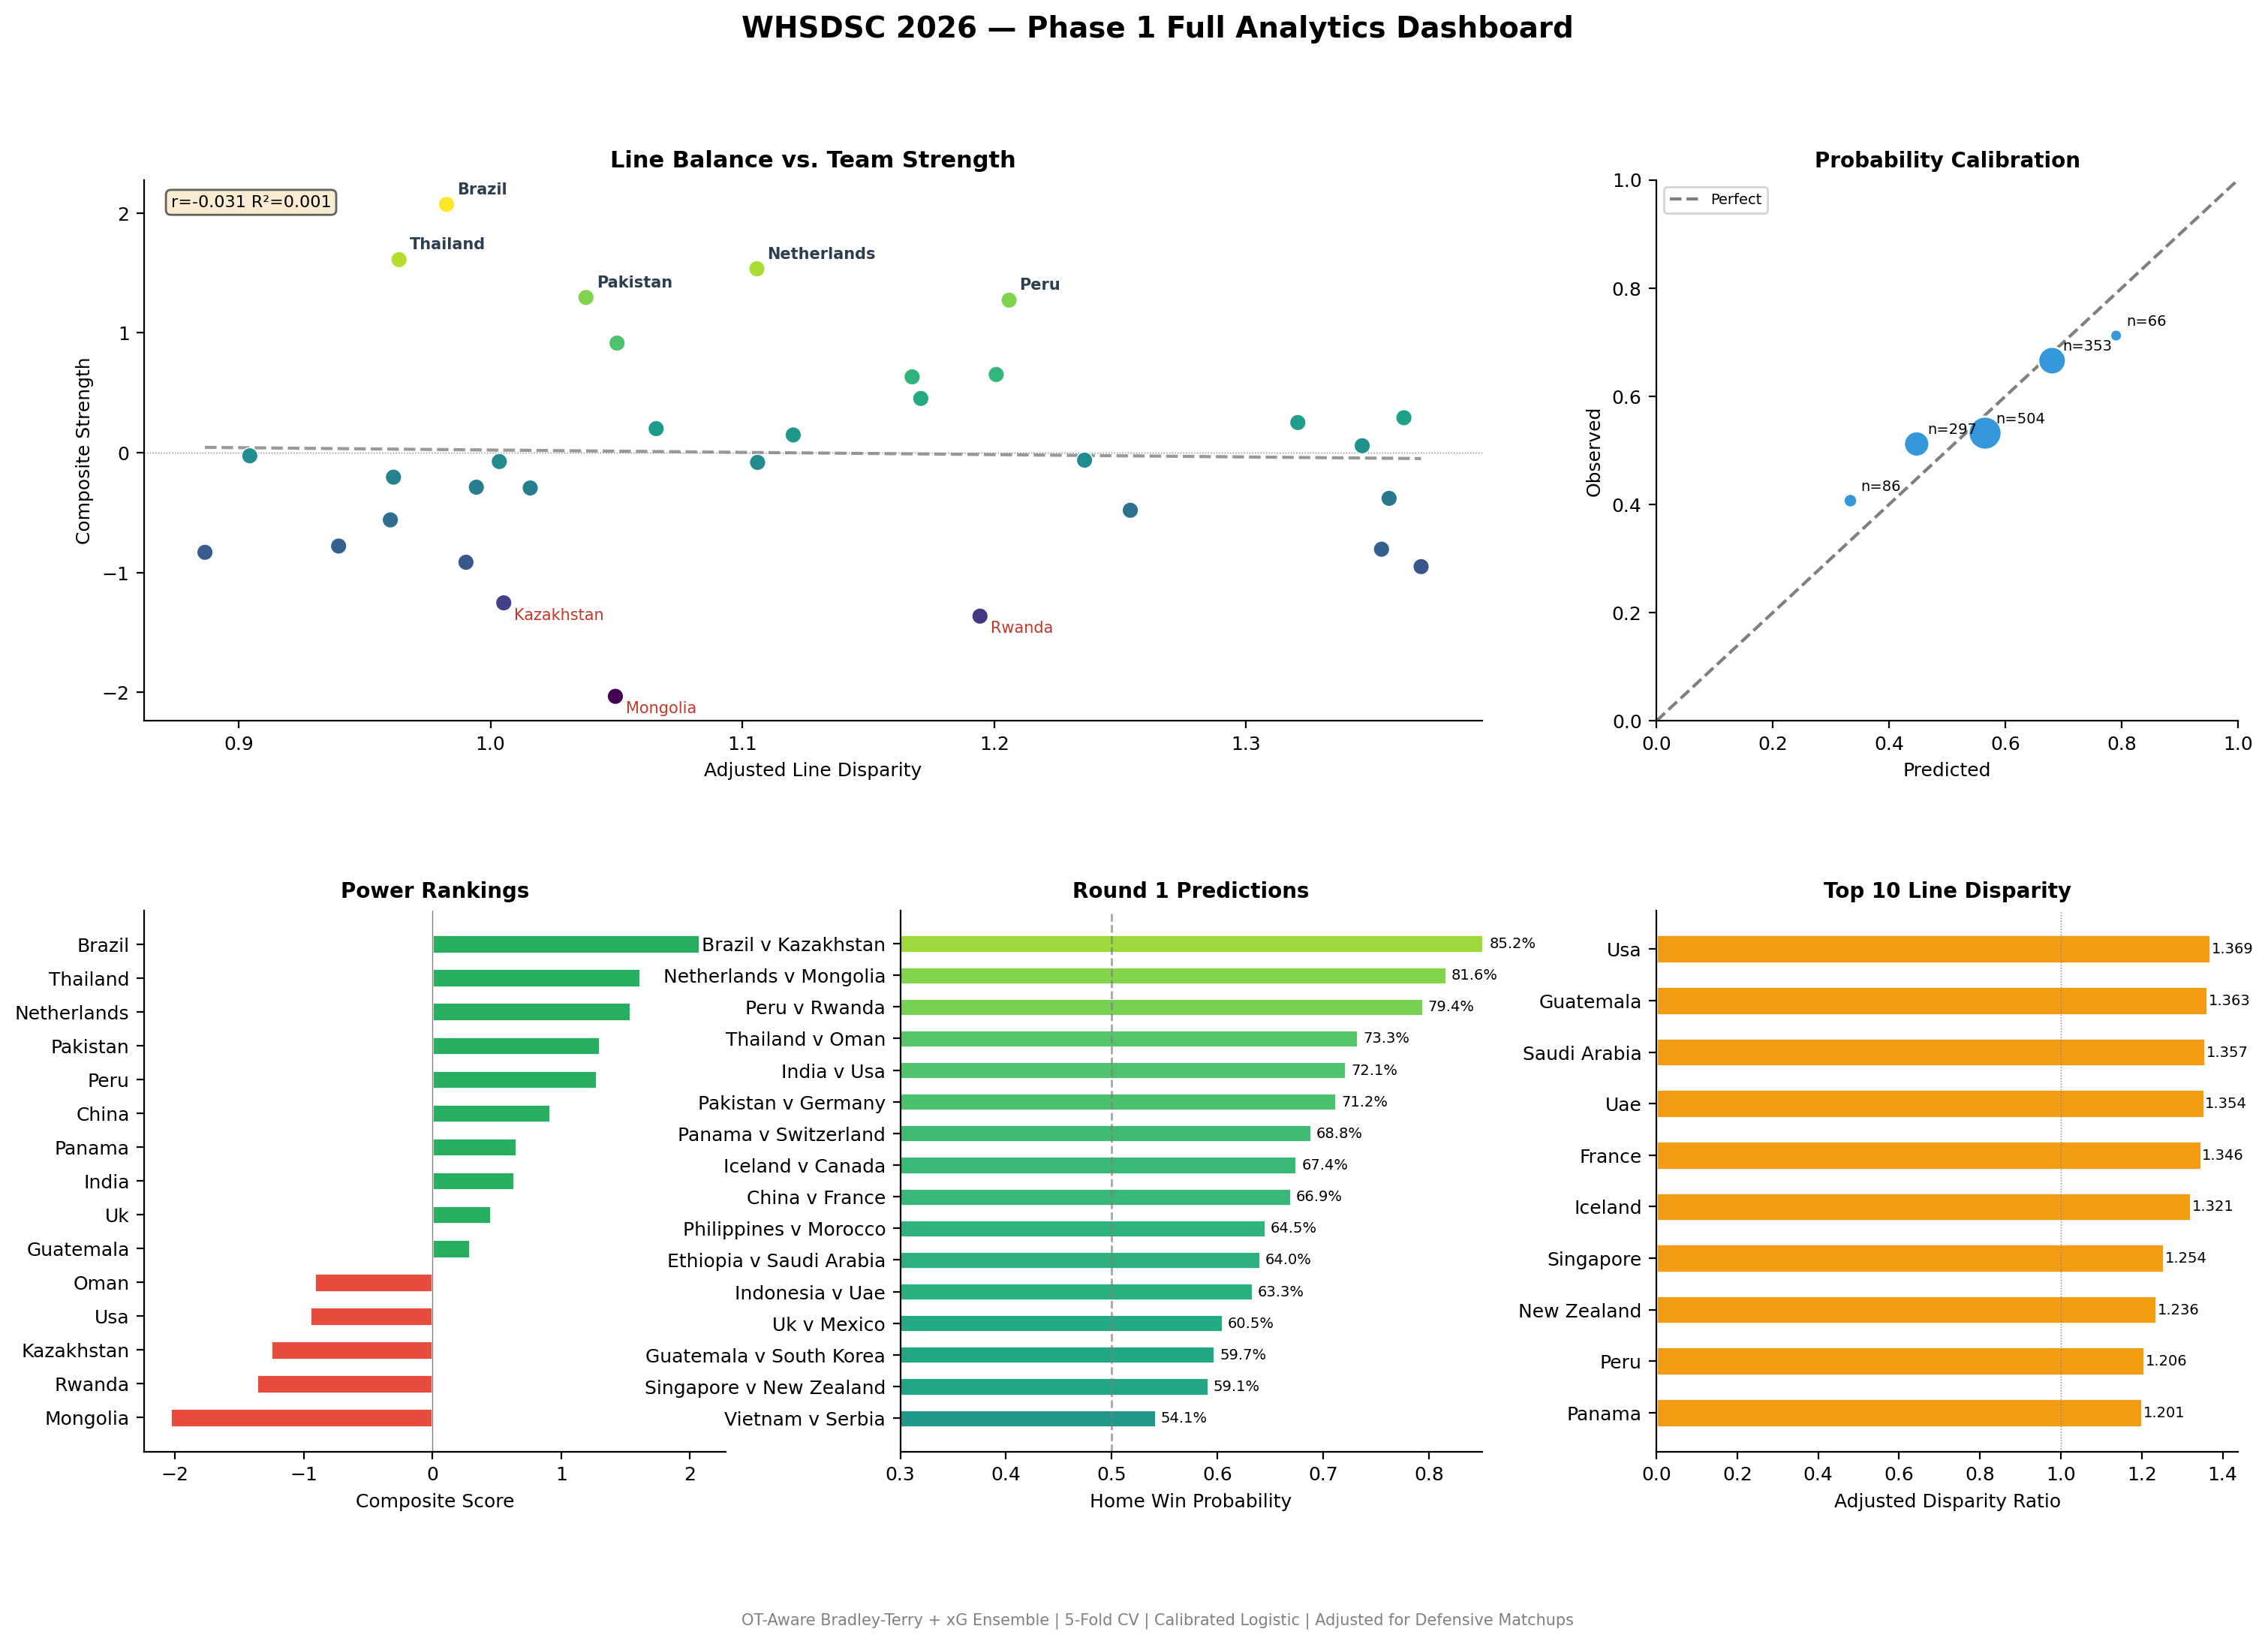
\includegraphics[width=\textwidth]{../output/submission/dashboard.png}
    \caption{完整分析仪表盘：（左上）阵容均衡 vs.\ 实力散点图，（右上）校准曲线，（左下）实力排名柱状图，（中下）第一轮对决预测，（右下）前 10 进攻线差异。}
    \label{fig:dashboard}
\end{figure}

% ═════════════════════════════════════════════════════════════
\section{ML 模型对比实验}
\label{sec:ml}

除了最终采用的 BT 逻辑回归外，我们还测试了多种机器学习挑战者模型作为基准比较。图~\ref{fig:ml} 展示了完整的 ML 模型对比仪表盘。

\begin{figure}[H]
    \centering
    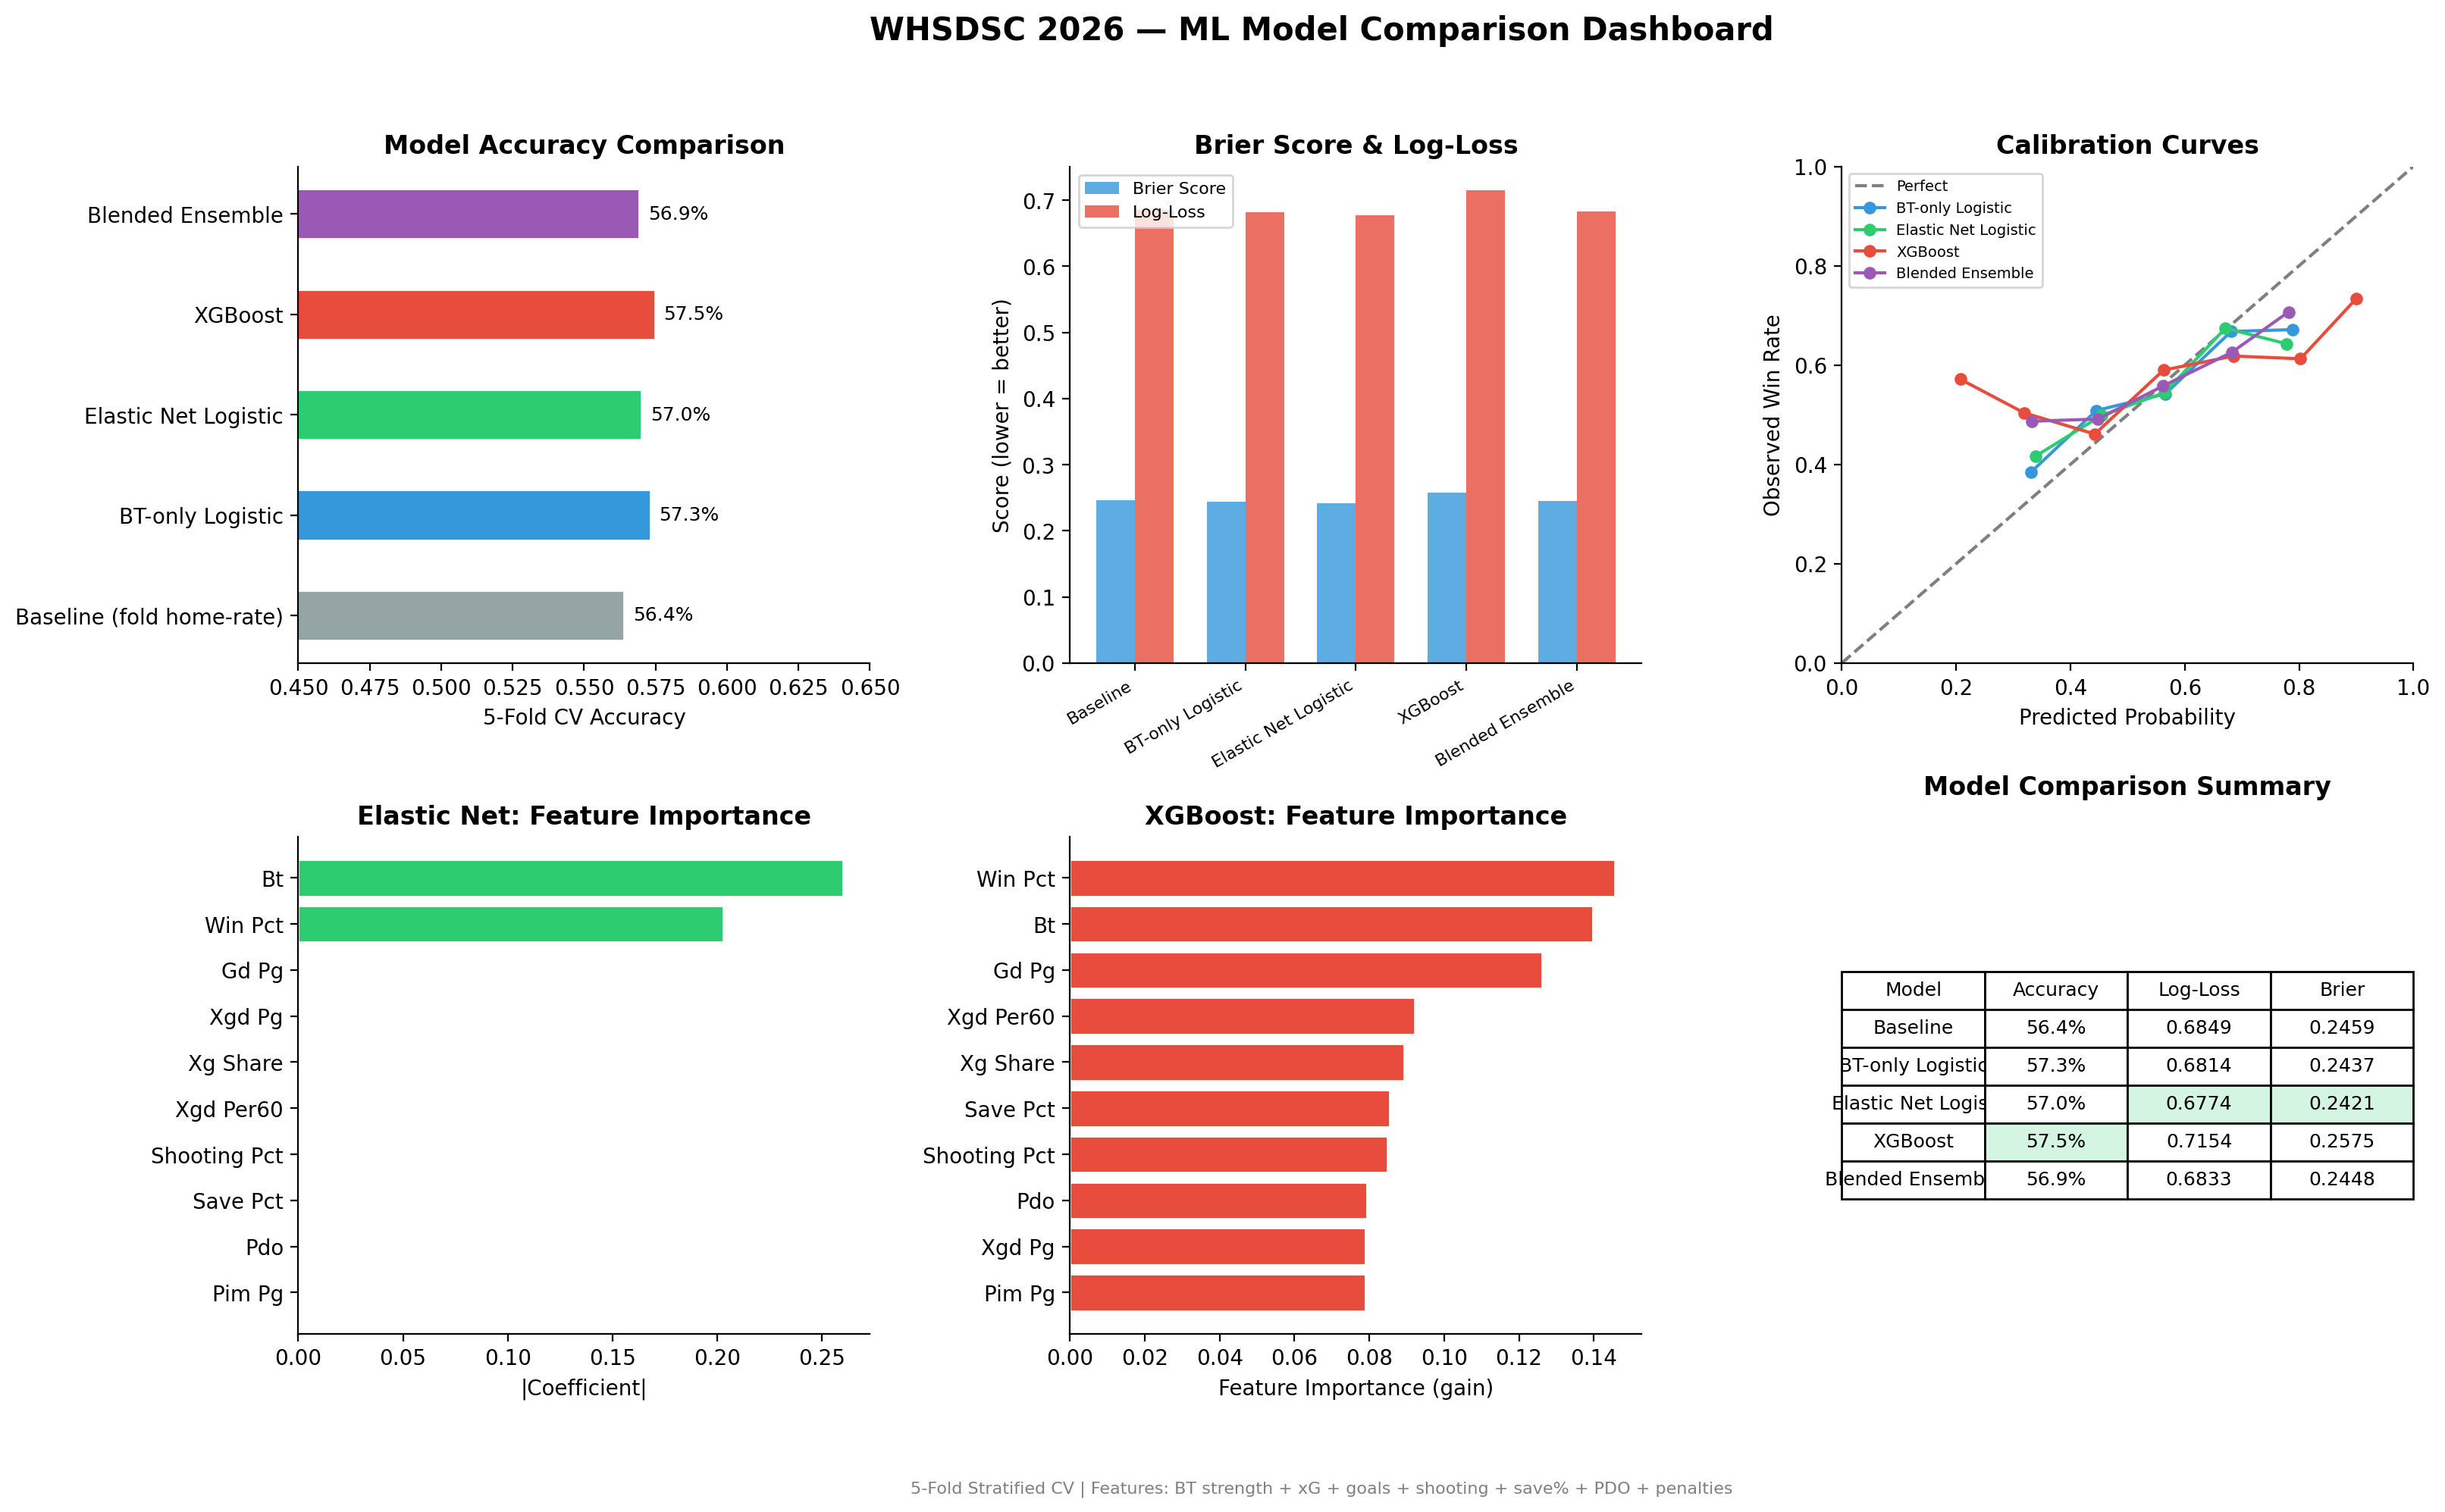
\includegraphics[width=\textwidth]{fig_ml_comparison.png}
    \caption{ML 模型对比仪表盘（6 面板）：（左上）5 折 CV 准确率对比——Elastic Net 58.0\% 最高，（中上）Brier 分数与 Log-Loss 对比，（右上）各模型校准曲线，（左下/中下）Elastic Net 与 XGBoost 特征重要性，（右下）汇总表。总体上复杂 ML 在随机 CV 中可带来边际提升，但稳健性与可解释性仍需权衡。}
    \label{fig:ml}
\end{figure}

\noindent\textbf{关键发现}：
\begin{itemize}[nosep]
    \item \textbf{随机 CV 下最佳准确率}：Elastic Net 达到 58.0\%，同时 Log-Loss 0.6758、Brier 0.2412 也最优；但其复杂度与特征依赖高于 BT-only 模型。
    \item \textbf{XGBoost 仍存在校准问题}：准确率 56.7\%，Log-Loss 0.7157、Brier 0.2574，作为概率输出模型明显偏弱。
    \item \textbf{BT-only 仍是强基线}：OT-aware BT 逻辑回归（57.0\%，Log-Loss 0.6796，Brier 0.2430）在可解释性与稳定性上更适合作为正式提交模型；混合集成（57.8\%，Brier 0.2443）并未在概率质量上超过 Elastic Net。
    \item 特征重要性（基于全量数据重拟合、仅用于解释）显示 \textbf{BT 与胜率差等汇总实力特征}均位于前列，复杂模型主要在这些信号上做非线性重加权。
    \item 因此最终提交仍采用 \textbf{OT-aware BT + 校准逻辑回归}，优先考虑\textbf{可解释性和稳定校准}（见第~\ref{sec:logistic} 节）。
\end{itemize}

% ═════════════════════════════════════════════════════════════
\section{描述性特征探索}
\label{sec:descriptive}

我们探索了数据集中三个未用于预测的额外特征：

\subsection{门将表现 (GSAx)}
\textbf{预期失球以上扑救数}（GSAx/场）= $(\text{xGA} - \text{GA}) / \text{场次}$。正值表示门将扑出了超过预期的射门。GSAx 与 BT 实力的相关系数 $r = 0.64$——强队通常拥有强门将，因此将 GSAx 加入逻辑回归\textbf{不增加任何准确率}。

\subsection{射门质量 (xG/Shot)}
每次射门的平均期望进球衡量进攻质量。与 BT 的相关性 $r = 0.48$。在挑战者实验中加入该特征后，\textbf{概率质量指标（Brier/Log-Loss）未见改善且可能略有恶化}，因此仅作为描述性分析保留。

\subsection{纪律性 (PIM/G，罚球差)}
通过每场罚时分钟数和罚球净值衡量球队纪律性。与 BT 的相关性 $r = 0.10$（弱）。\textbf{无预测提升。}

\textbf{结论}：三个特征均被 \textbf{BT 模型大量吸收}——球队的胜负记录已经捕获了门将质量、射门质量和纪律性的下游效应。我们将其作为描述性列报告在排名 CSV 中，但不纳入预测模型，防止过拟合。

% ═════════════════════════════════════════════════════════════
\section{AI 协作}
\label{sec:ai}

三个 AI 助手在项目中提供了独立视角：

\begin{table}[H]
\centering
\caption{AI 协作分工}
\begin{tabular}{ll}
\toprule
\textbf{AI} & \textbf{贡献} \\
\midrule
\textbf{Claude}（Anthropic） & 核心流水线设计、特征工程、BT 实现、深度验证（22 项检查清单） \\
\textbf{Gemini}（Google） & 审查排名、建议门将/特勤特征、校准评审 \\
\textbf{Codex}（OpenAI, GPT-5.3） & ML 挑战者验证、Brier 分数报告、88K token 代码审查（8.5/10 评分） \\
\bottomrule
\end{tabular}
\end{table}

\noindent 所有输出均经过跨模型交叉验证；最终方法论决策由人类主导。

% ═════════════════════════════════════════════════════════════
\section{局限性与未来工作}
\label{sec:limitations}

\begin{enumerate}
    \item \textbf{球队实力静态假设}：我们将球队实力视为赛季内恒定。现实中球队会因交易、伤病和势头而变化。时间衰减加权（如指数衰减）可以改善，但数据集未提供日期/场序信息。

    \item \textbf{高端过度自信}：校准显示预测概率超过 75\% 时，实际偏乐观约 8 个百分点（预测 0.79，实际 0.71）。折外保序回归 (isotonic calibration) 可缓解此问题。

    \item \textbf{冰球的固有随机性}：我们当前 57.0\% 的交叉验证准确率与冰球的高随机性特征一致。冰球是四大职业联赛中单场得分最低的运动，使得单场预测存在根本性限制。

    \item \textbf{无球员级建模}：我们将球队视为整体。纳入球员级数据（如 WAR、Corsi）可提升精细度，但数据集未提供。

    \item \textbf{主场优势假设统一}：我们对所有球队使用单一主场参数 $\alpha$。实际中不同场馆的主场优势程度不同。
\end{enumerate}

% ═════════════════════════════════════════════════════════════
\section{结论}
\label{sec:conclusion}

我们构建了一个原则性强、透明且可复现的冰球分析框架：

\begin{itemize}
    \item \textbf{加时赛感知 Bradley-Terry 模型}：正确地将加时赛胜利视为较弱的信号。
    \item \textbf{校准逻辑回归}：提供可解释的胜率预测，配合诚实的折外评估。
    \item \textbf{防守分层校正的进攻线差异指标}：控制了 1 对/2 对对位层级带来的主要混杂因素。
    \item 明确发现\textbf{进攻线均衡度与球队成功之间不存在显著关系}（$r = -0.031$）。
\end{itemize}

该模型优先考虑\textbf{可解释性而非边际精度提升}：领域专家可以审查从原始数据到最终预测的每一个步骤。这种透明性是本方案最大的优势。

\vspace{0.5cm}
\hrule
\vspace{0.3cm}
\begin{center}
\small\textit{WHSDSC 2026 $\cdot$ 第一阶段 $\cdot$ Claude + Gemini + Codex 交叉验证}
\end{center}

\end{document}
